\documentclass{beamer}
%Information to be included in the title page:
\title{Piecewise Linear Function}
\subtitle{with discontinuity at $x = 0$}
\author{Fabian Weik}
\date{\today}

\usepackage{listings}

\graphicspath{{../../Simulation/Models/00_Examples/05_Homework_0124}}

\usepackage{forloop}
\usepackage{calc}
\newcounter{n}
\newcounter{f}
\makeatletter
\newcommand{\twodigits}{\two@digits}
\makeatother

\usepackage{subfig}

\begin{document}

\frame{\titlepage}

\begin{frame}[fragile]{Code}
    \begin{lstlisting}
real_t x = currentState[0];
real_t y = 0;

if (x < 0) {
    y = aL * x + mu;
} else {
    y = aR * x + mu;
}

RHS[0] = y;
return true;
    \end{lstlisting}
    
    Executed using AnT
    
\end{frame}

\begin{frame}{(i.a) $a_L = -1, a_R = 2$}
    \begin{figure}
        \centering
        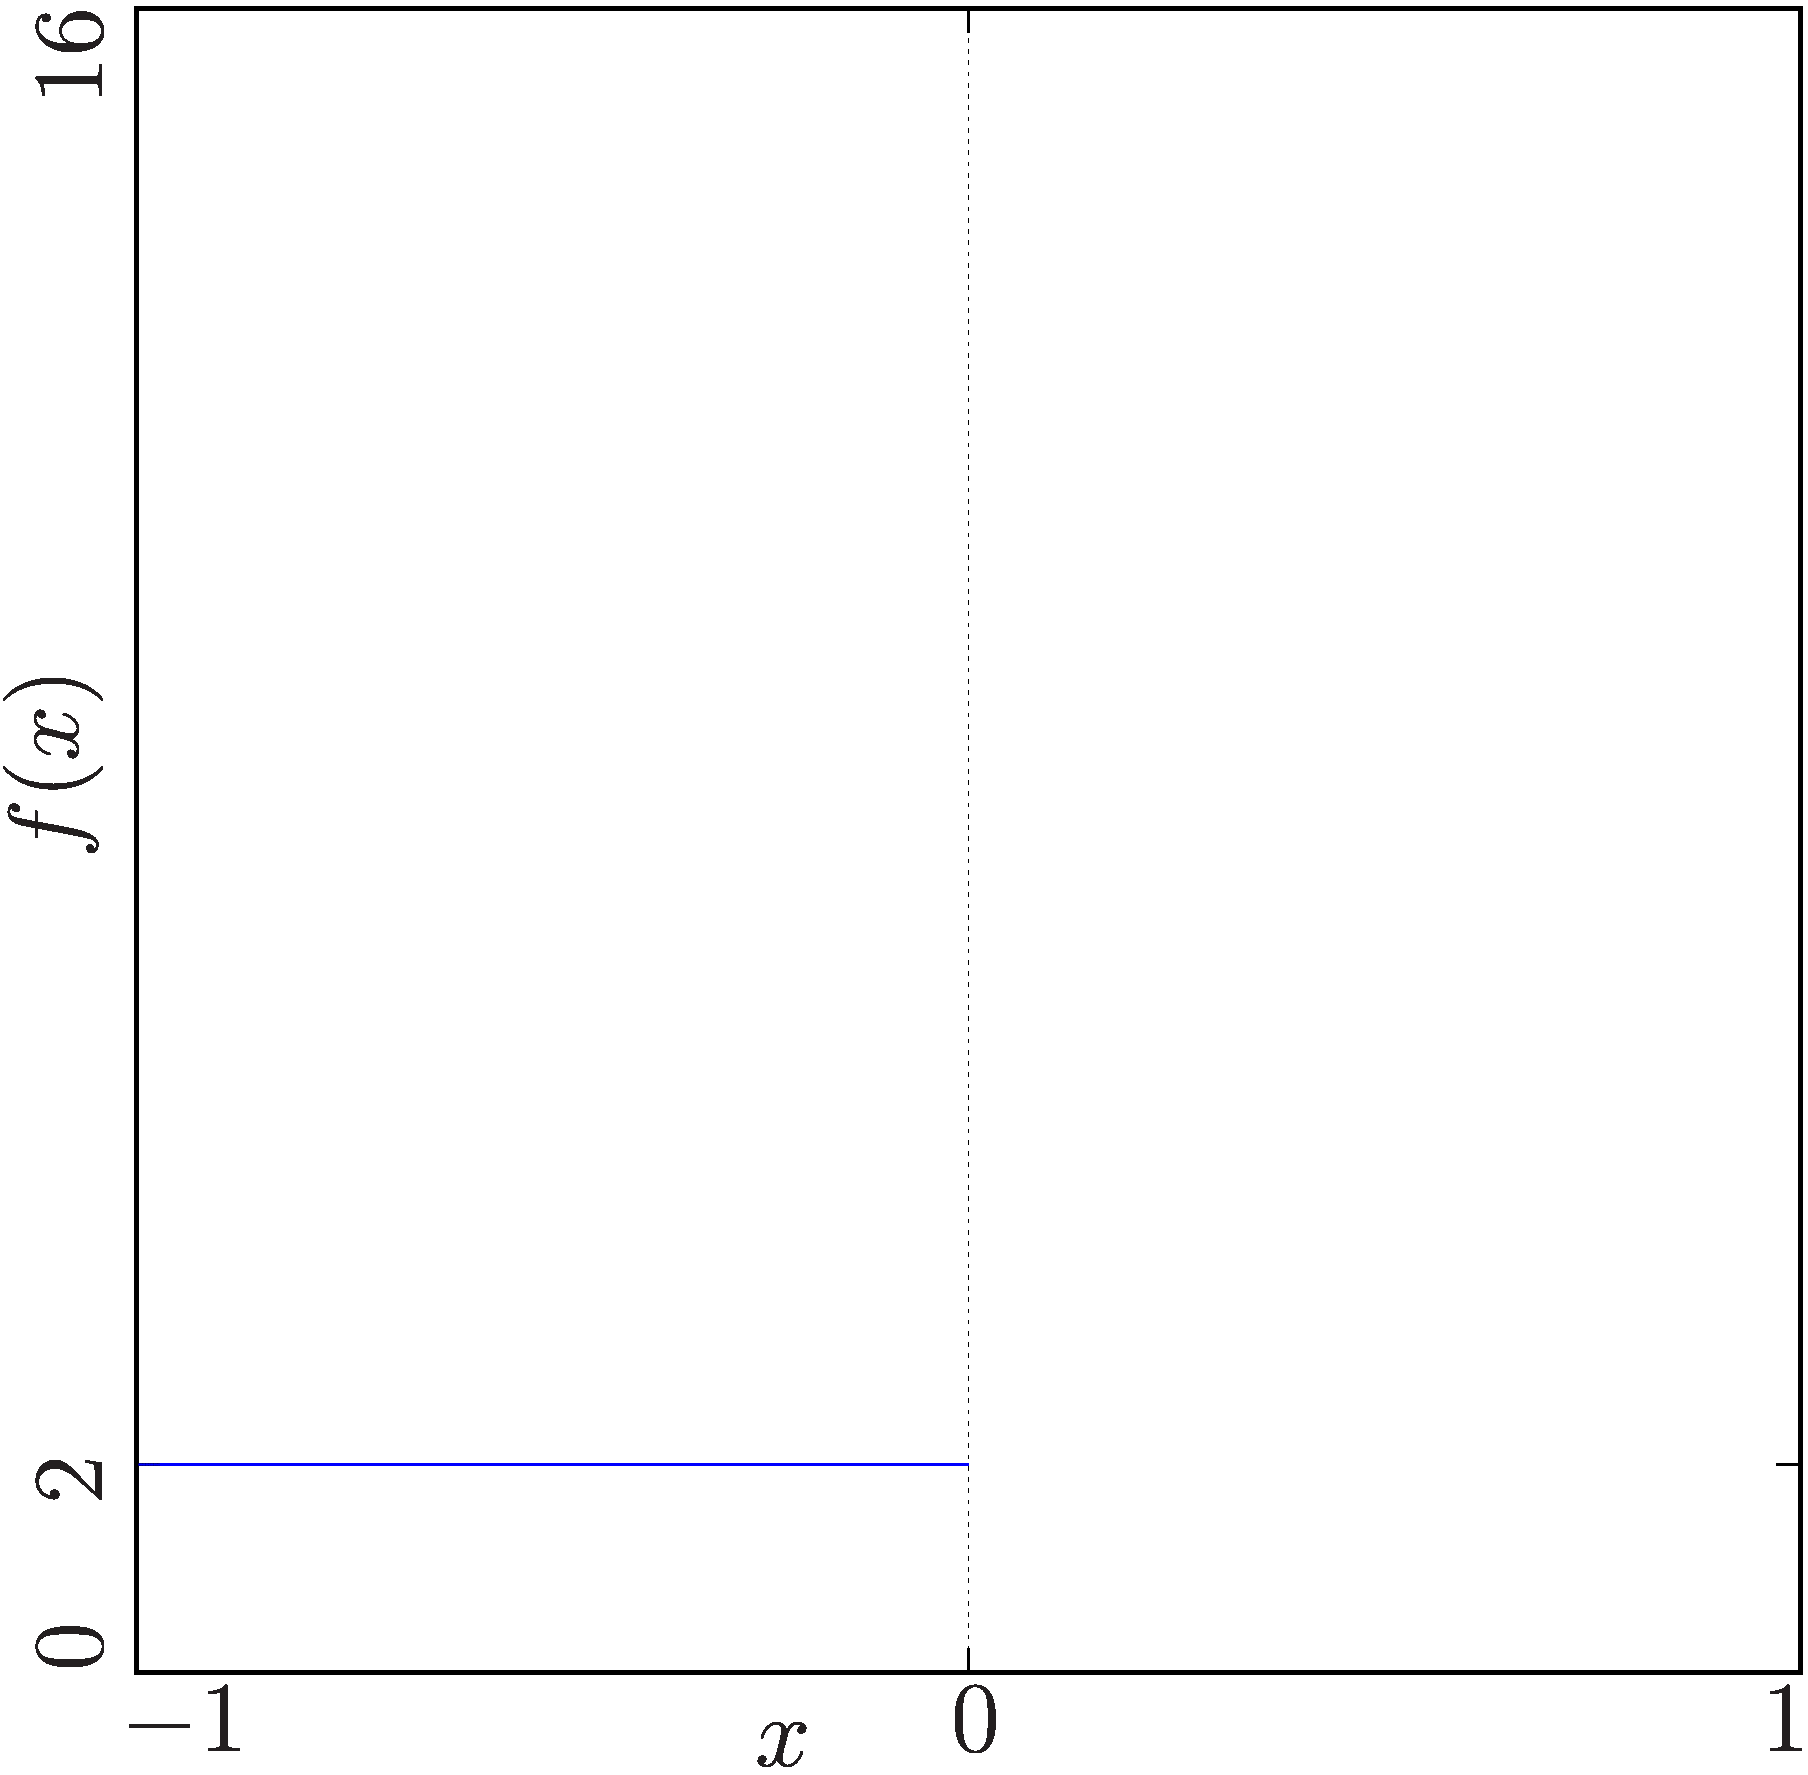
\includegraphics[width=0.6\textwidth]{1D_i/result.png}
        \caption{Varying $\mu$}
    \end{figure}
\end{frame}

\begin{frame}{(i.a) $a_L = -1, a_R = 2$}
    \begin{figure}
        \centering
            \forloop{n}{0}{\value{n} < 5}{
                \setcounter{f}{\value{n}+1}
                \includegraphics<\arabic{f}>[width=0.6\textwidth]{
                    Cob_i/Autogen/Frame_00\twodigits{\value{n}}/result.png
                }
            }
        \caption{Cobwebs $\mu \in \{0.01, 0, -0.01, -0.02, -0.03\}$}
    \end{figure}
        
    $\mu < 0$: infinite unstable 2-cycles and one unstable fixpoint
    Absorbing interval: $(\mu, 0)$
\end{frame}

\begin{frame}{(i) What happens if we change $a_R$?}
    \begin{figure}
        \centering
        \subfloat[Initial State $-\epsilon$]{
            \includegraphics<1>[width=0.4\textwidth]{2D_i_aR/result.png}
            \includegraphics<2>[width=0.4\textwidth]{2D_i_aR_Zoomed/result.png}
        } \qquad
        \subfloat[Initial State $\epsilon$]{
            \includegraphics<1>[width=0.4\textwidth]{2D_i_aRp/result.png}
            \includegraphics<2>[width=0.4\textwidth]{2D_i_aRp_Zoomed/result.png}
        }
        \caption{Varying $a_R$}
    \end{figure}
    
    blue/black: no cycle
    \hspace*{\fill}
    pink: fixed point
    \hspace*{\fill}
    white: 2-cycle
\end{frame}

\begin{frame}{(i) what happens if we change $a_R$?}
    Not yet seen dynamics:
    \begin{enumerate}
        \item[(0.a)] No cyclic behavior to 2-cycle for $a_R \in [1, \infty) \cup (-\infty, -1)$
        \item[(0.b)] Fixpoint to 2-cycle for $a_R \in (-1, 1)$
        \item[(0.c)] 2-cycle stays for $a_R = -1$
    \end{enumerate}
\end{frame}

\begin{frame}{(i.b) $a_L = -1, a_R = 0.5$}
    \begin{figure}
        \centering
        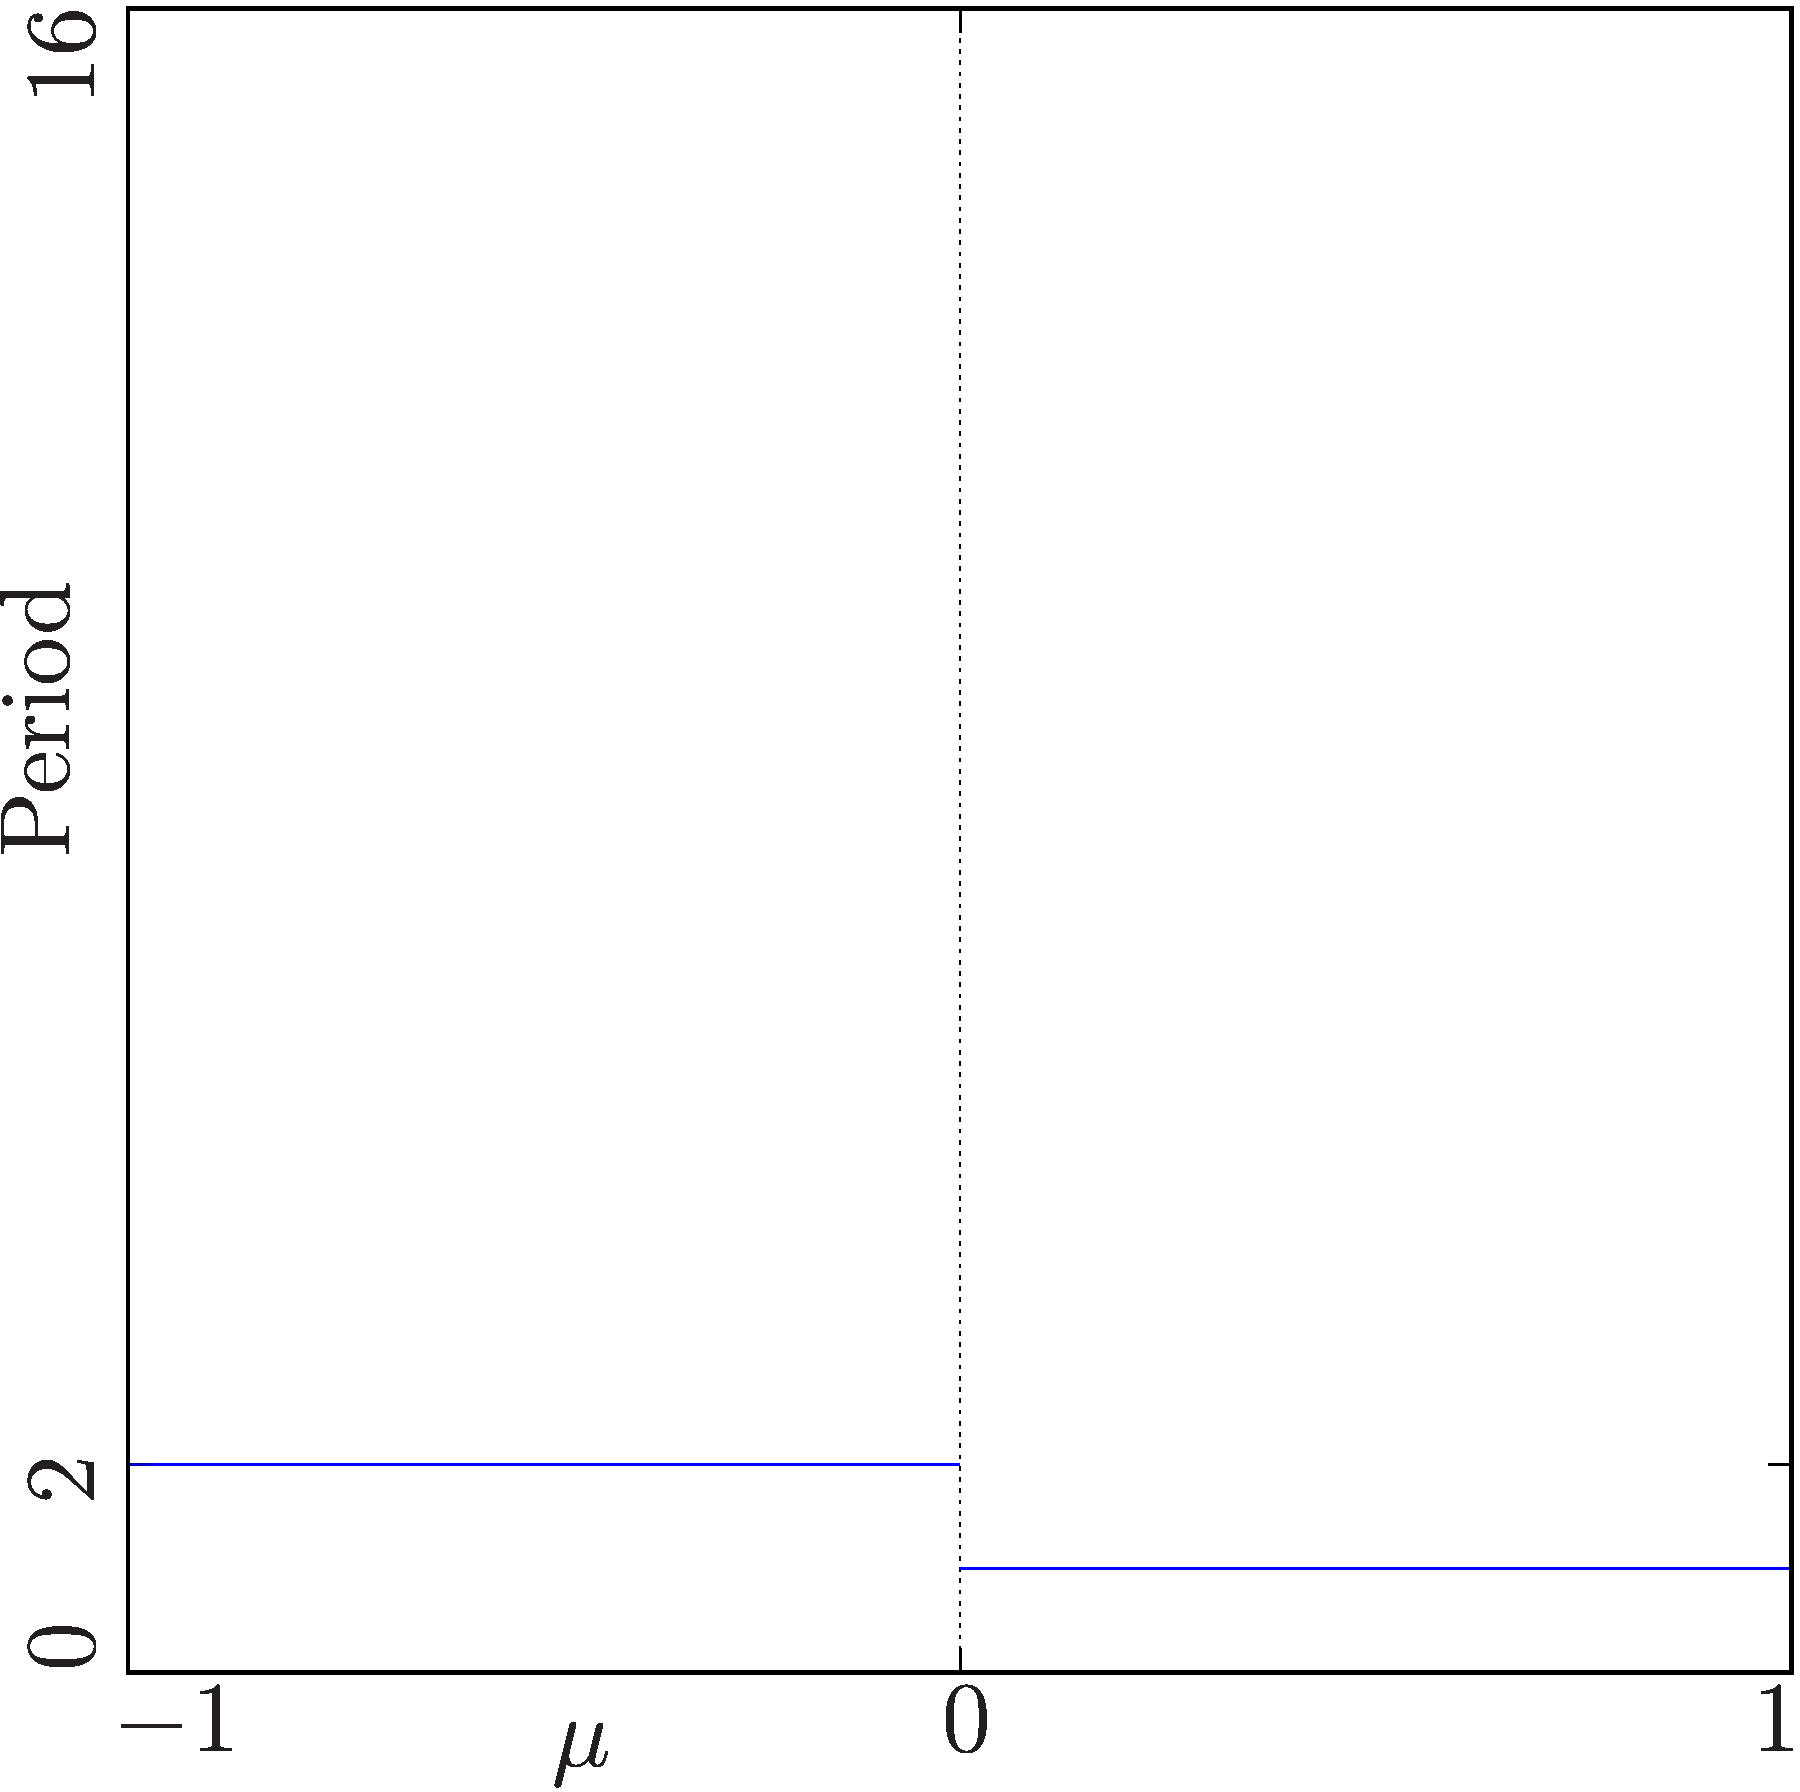
\includegraphics[width=0.6\textwidth]{1D_ib/result.png}
        \caption{Varying $\mu$}
    \end{figure}
\end{frame}

\begin{frame}{(i.b) $a_L = -1, a_R = 0.5$}
    \begin{figure}
        \centering
            \forloop{n}{0}{\value{n} < 5}{
                \setcounter{f}{\value{n}+1}
                \includegraphics<\arabic{f}>[width=0.5\textwidth]{
                    Cob_ib/Autogen/Frame_00\twodigits{\value{n}}/result.png
                }
            }
        \caption{Cobwebs $\mu \in \{0.02, 0.01, 0, -0.01, -0.02\}$}
    \end{figure}
        
    Absorbing interval: $(-\infty, \infty)$
        
    $\mu >= 0$: stable fixpoint at $2 \mu$, \\
    $\mu < 0$: infinite unstable 2-cycles and one unstable fixpoint
\end{frame}

\begin{frame}{(i.c) $a_L = a_R = -1$ (Not a bifurcation)}
    \begin{figure}
        \centering
        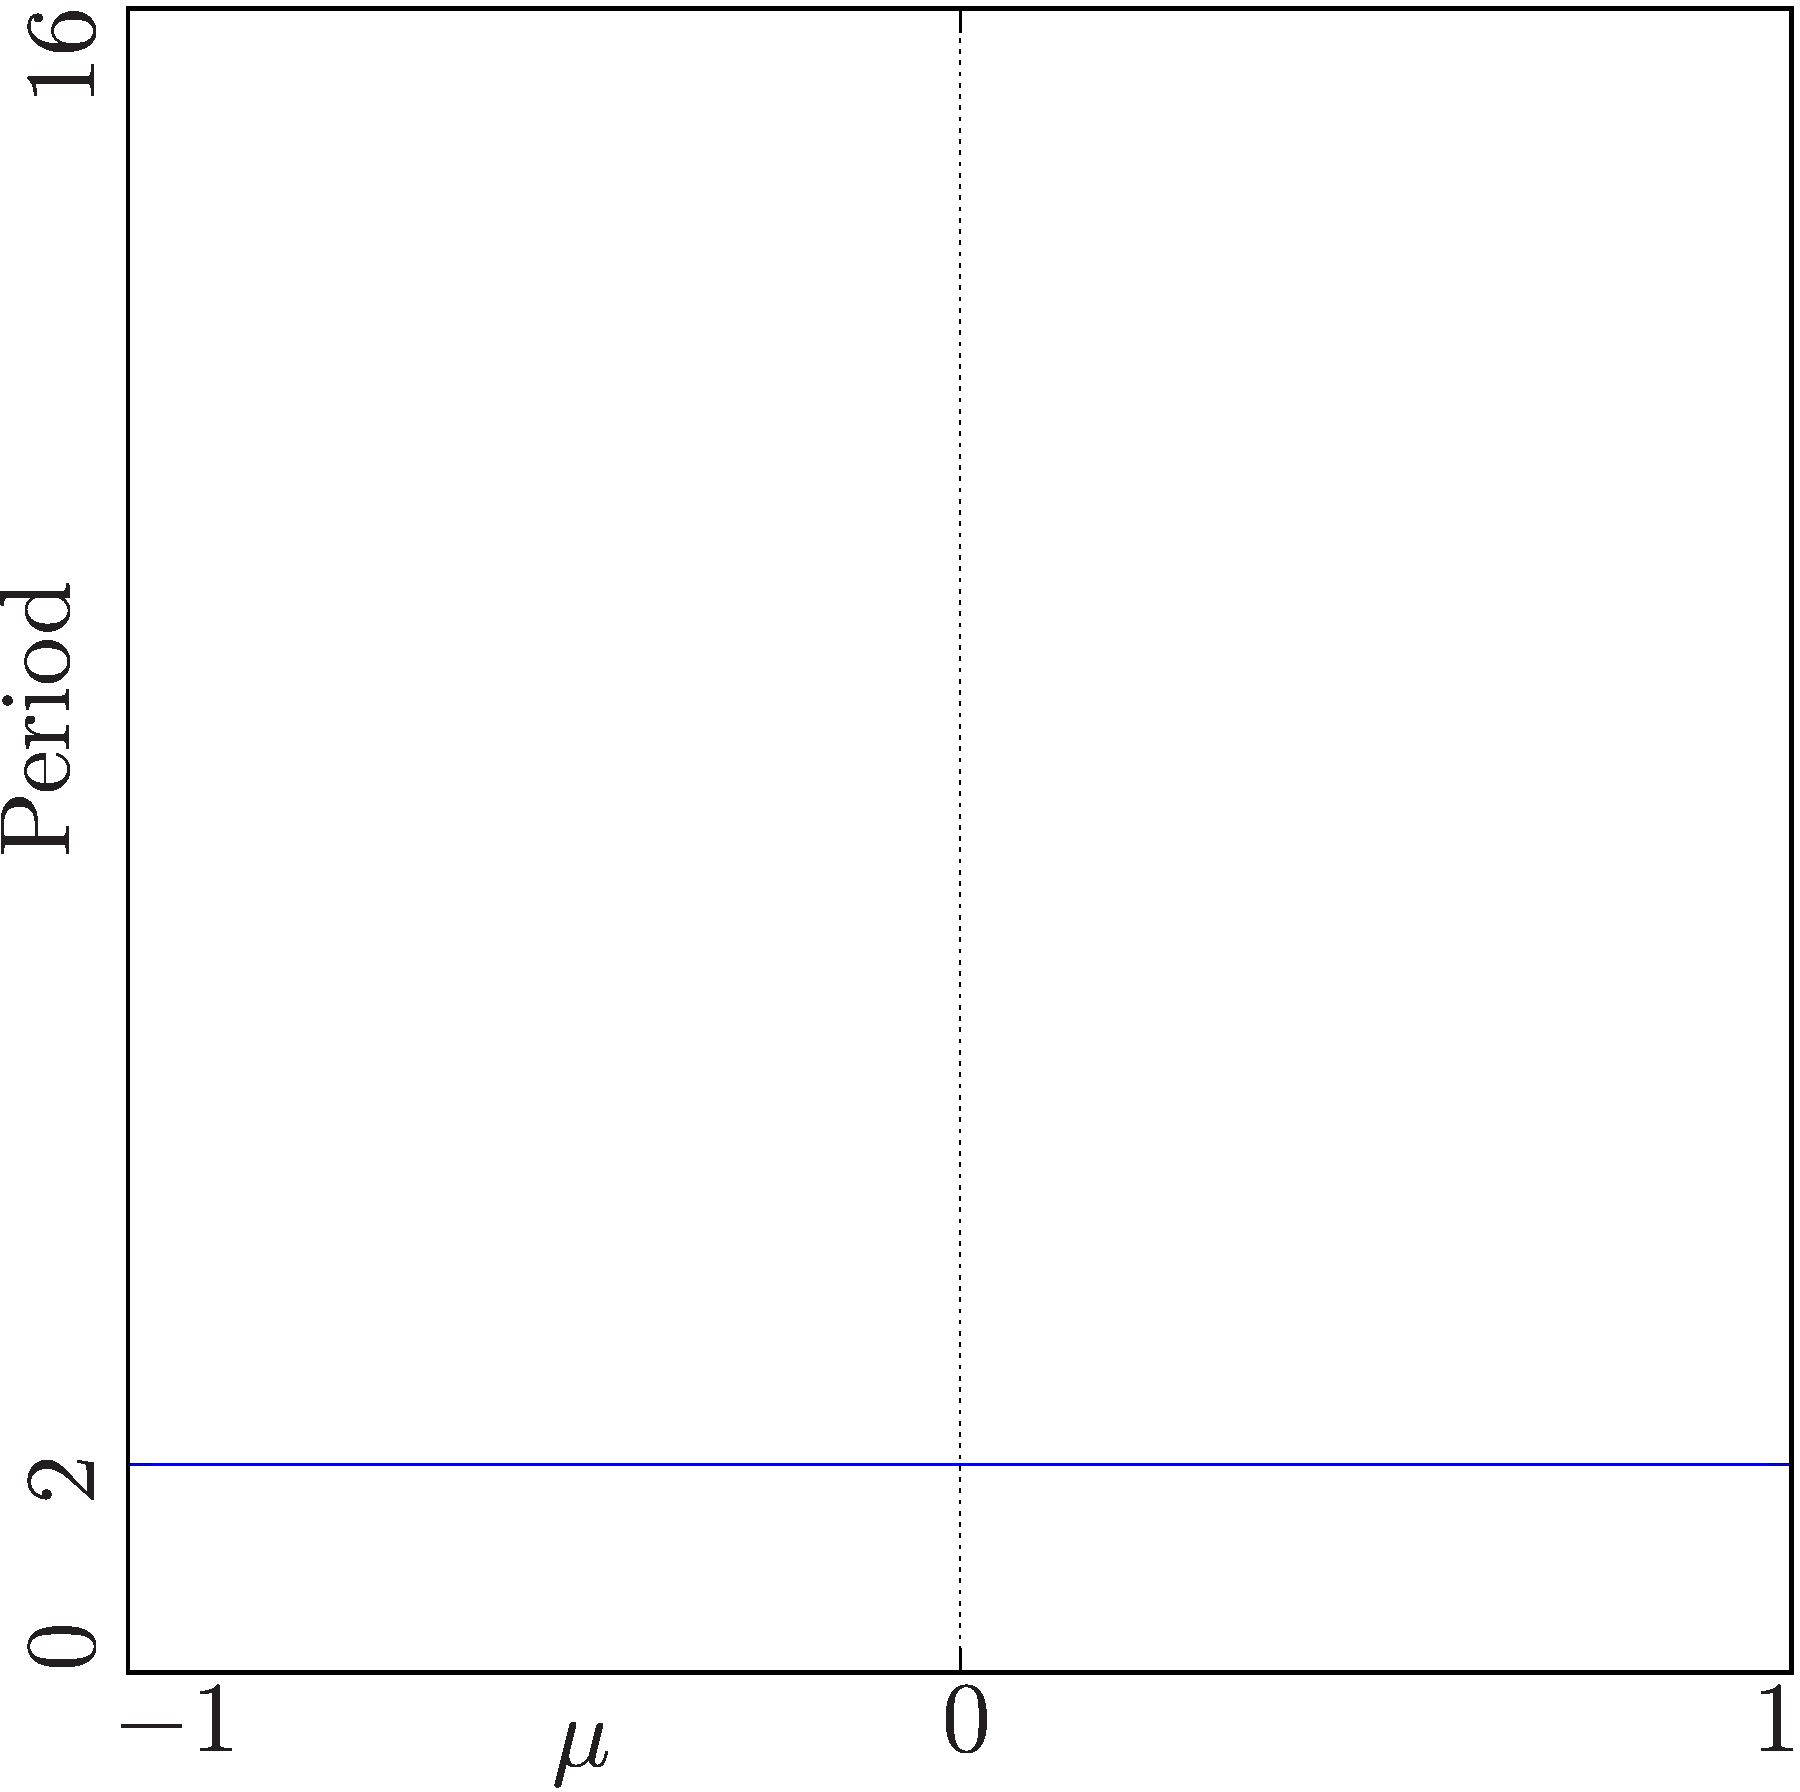
\includegraphics[width=0.6\textwidth]{1D_ic/result.png}
        \caption{Varying $\mu$}
    \end{figure}
\end{frame}

\begin{frame}{(i.c) $a_L = a_R = -1$ (Not a bifurcation)}
    \begin{figure}
        \centering
            \forloop{n}{0}{\value{n} < 5}{
                \setcounter{f}{\value{n}+1}
                \includegraphics<\arabic{f}>[width=0.6\textwidth]{
                    Cob_ic/Autogen/Frame_00\twodigits{\value{n}}/result.png
                }
            }
        \caption{Cobwebs $\mu \in \{0.02, 0.01, 0, -0.01, -0.02\}$}
    \end{figure}
    
    Infinite unstable 2-cycles everywhere plus one fixpoint at $\frac{\mu}{2}$
\end{frame}

\begin{frame}{(i.a) What happens if we change $a_L$?}
    \begin{figure}
        \centering
        \subfloat[Initial State $-\epsilon$]{
            \includegraphics<1>[width=0.4\textwidth]{2D_i_aL/result.png}
            \includegraphics<2>[width=0.4\textwidth]{2D_i_aL_Zoomed/result.png}
        } \qquad
        \subfloat[Initial State $\epsilon$]{
            \includegraphics<1>[width=0.4\textwidth]{2D_i_aLp/result.png}
            \includegraphics<2>[width=0.4\textwidth]{2D_i_aLp_Zoomed/result.png}
        }
        \caption{Varying $a_L$}
    \end{figure}

    blue/black: no cycle
    \hspace*{\fill}
    pink: fixed point
    \hspace*{\fill}
    white: 2-cycle
\end{frame}

\begin{frame}{(0) Fix $a_L = -2$}
    Different dynamic for $a_L = -2$ from $a_L = -1$
\end{frame}

\begin{frame}{(0) what happens if we change $a_R$?}
    \begin{figure}
        \centering
        \subfloat[Initial State $-\epsilon$]{
            \includegraphics<1>[width=0.4\textwidth]{2D_0_aR/result.png}
            \includegraphics<2>[width=0.4\textwidth]{2D_0_aR_Zoomed/result.png}
        } \qquad
        \subfloat[Initial State $\epsilon$]{
            \includegraphics<1>[width=0.4\textwidth]{2D_0_aRp/result.png}
            \includegraphics<2>[width=0.4\textwidth]{2D_0_aRp_Zoomed/result.png}
        }
        \caption{Varying $a_R$}
    \end{figure}
    
    \hspace*{\fill}
    blue/black: no cycle
    \hspace*{\fill}
    purple: fixed point
    \hspace*{\fill}

    \hspace*{\fill}
    pink: 2-cycle
    \hspace*{\fill}
    white: 4-cycle
    \hspace*{\fill}
\end{frame}

\begin{frame}{(0) what happens if we change $a_R$?}
    Not yet seen dynamics:
    \begin{enumerate}
        \item[(0.a)] Fixpoint to no cyclic behaviour for $a_R \in (0.5, 1)$
        \item[(0.b)] Fixpoint to 4-cycle for $a_R = 0.5$
    \end{enumerate}

    \vspace*{2em}
    Already seen, but slightly different:
    \begin{enumerate}
        \item[(0.c)] Fixpoint to \textit{single} 2-cycle for $a_R \in (-0.5, 0.5)$
    \end{enumerate}
\end{frame}

\begin{frame}{(0.a) Fixing $a_L = -2, a_R = 0.75$}
    \begin{figure}
        \centering
        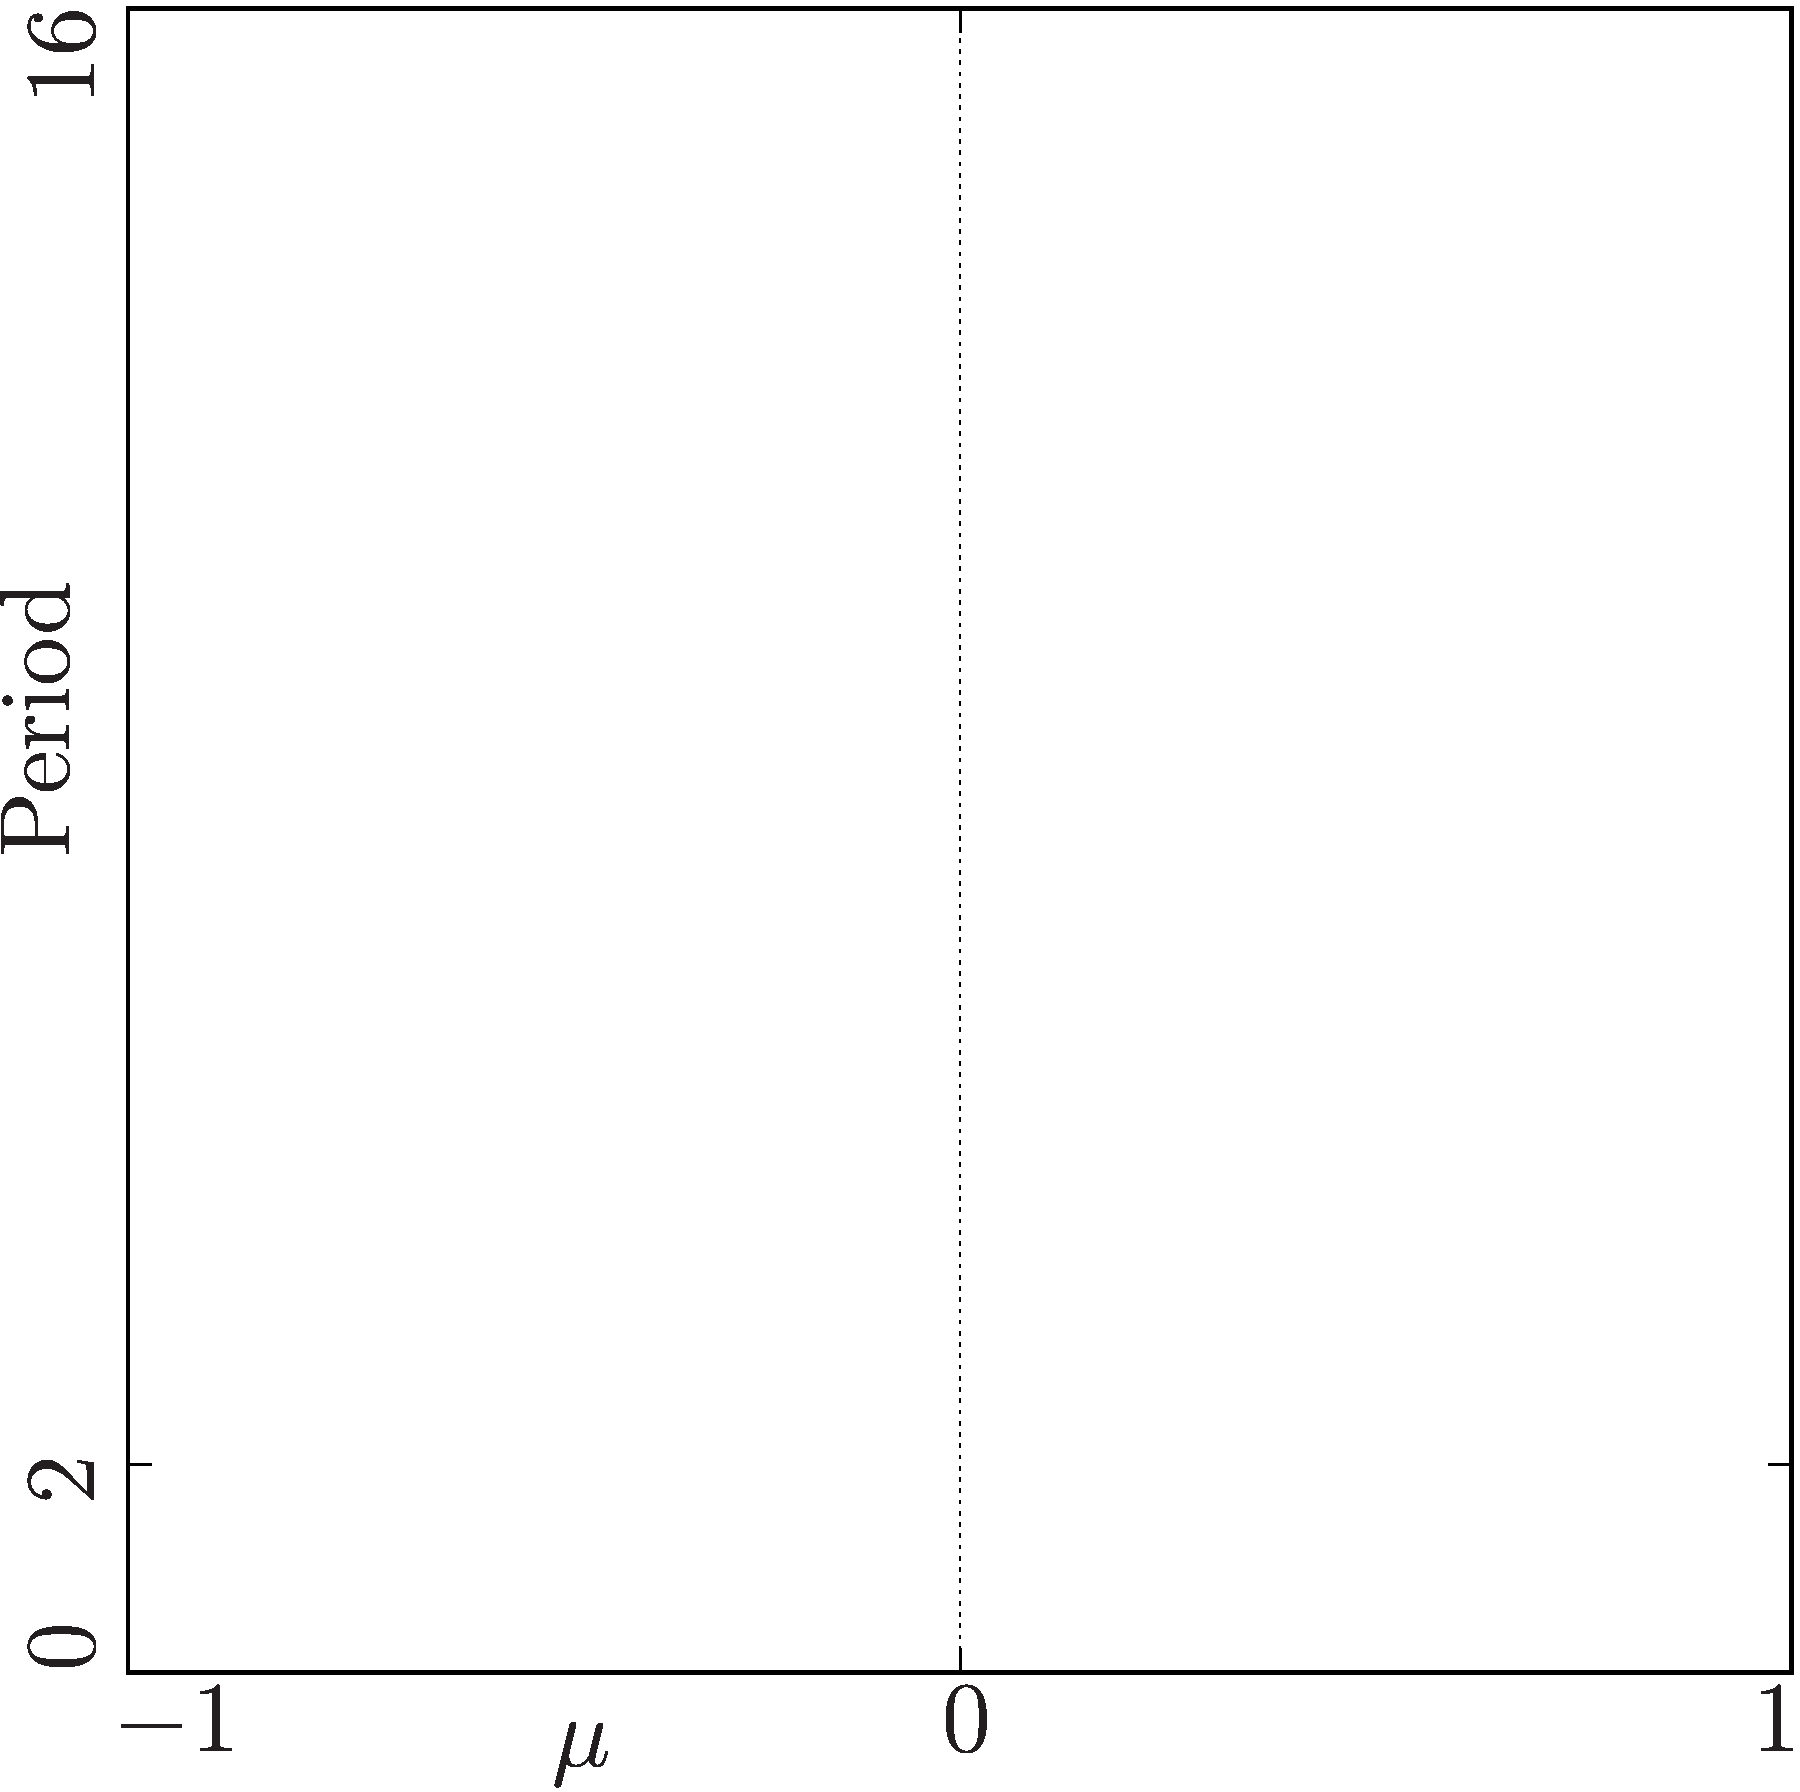
\includegraphics[width=0.6\textwidth]{1D_0a/result.png}
        \caption{Varying $\mu$}
    \end{figure}
\end{frame}

\begin{frame}{(0.a) Fixing $a_L = -2, a_R = 0.75$}
    \begin{figure}
        \centering
            \forloop{n}{0}{\value{n} < 5}{
                \setcounter{f}{\value{n}+1}
                \includegraphics<\arabic{f}>[width=0.6\textwidth]{
                    Cob_0a/Autogen/Frame_00\twodigits{\value{n}}/result.png
                }
            }
        \caption{Cobwebs $\mu \in \{0.02, 0.01, 0, -0.01, -0.02\}$}
    \end{figure}
    
    Absorbing interval: $(-\infty, \infty)$
\end{frame}

\begin{frame}{(0.b) Fixing $a_L = -2, a_R = 0.5$}
    \begin{figure}
        \centering
        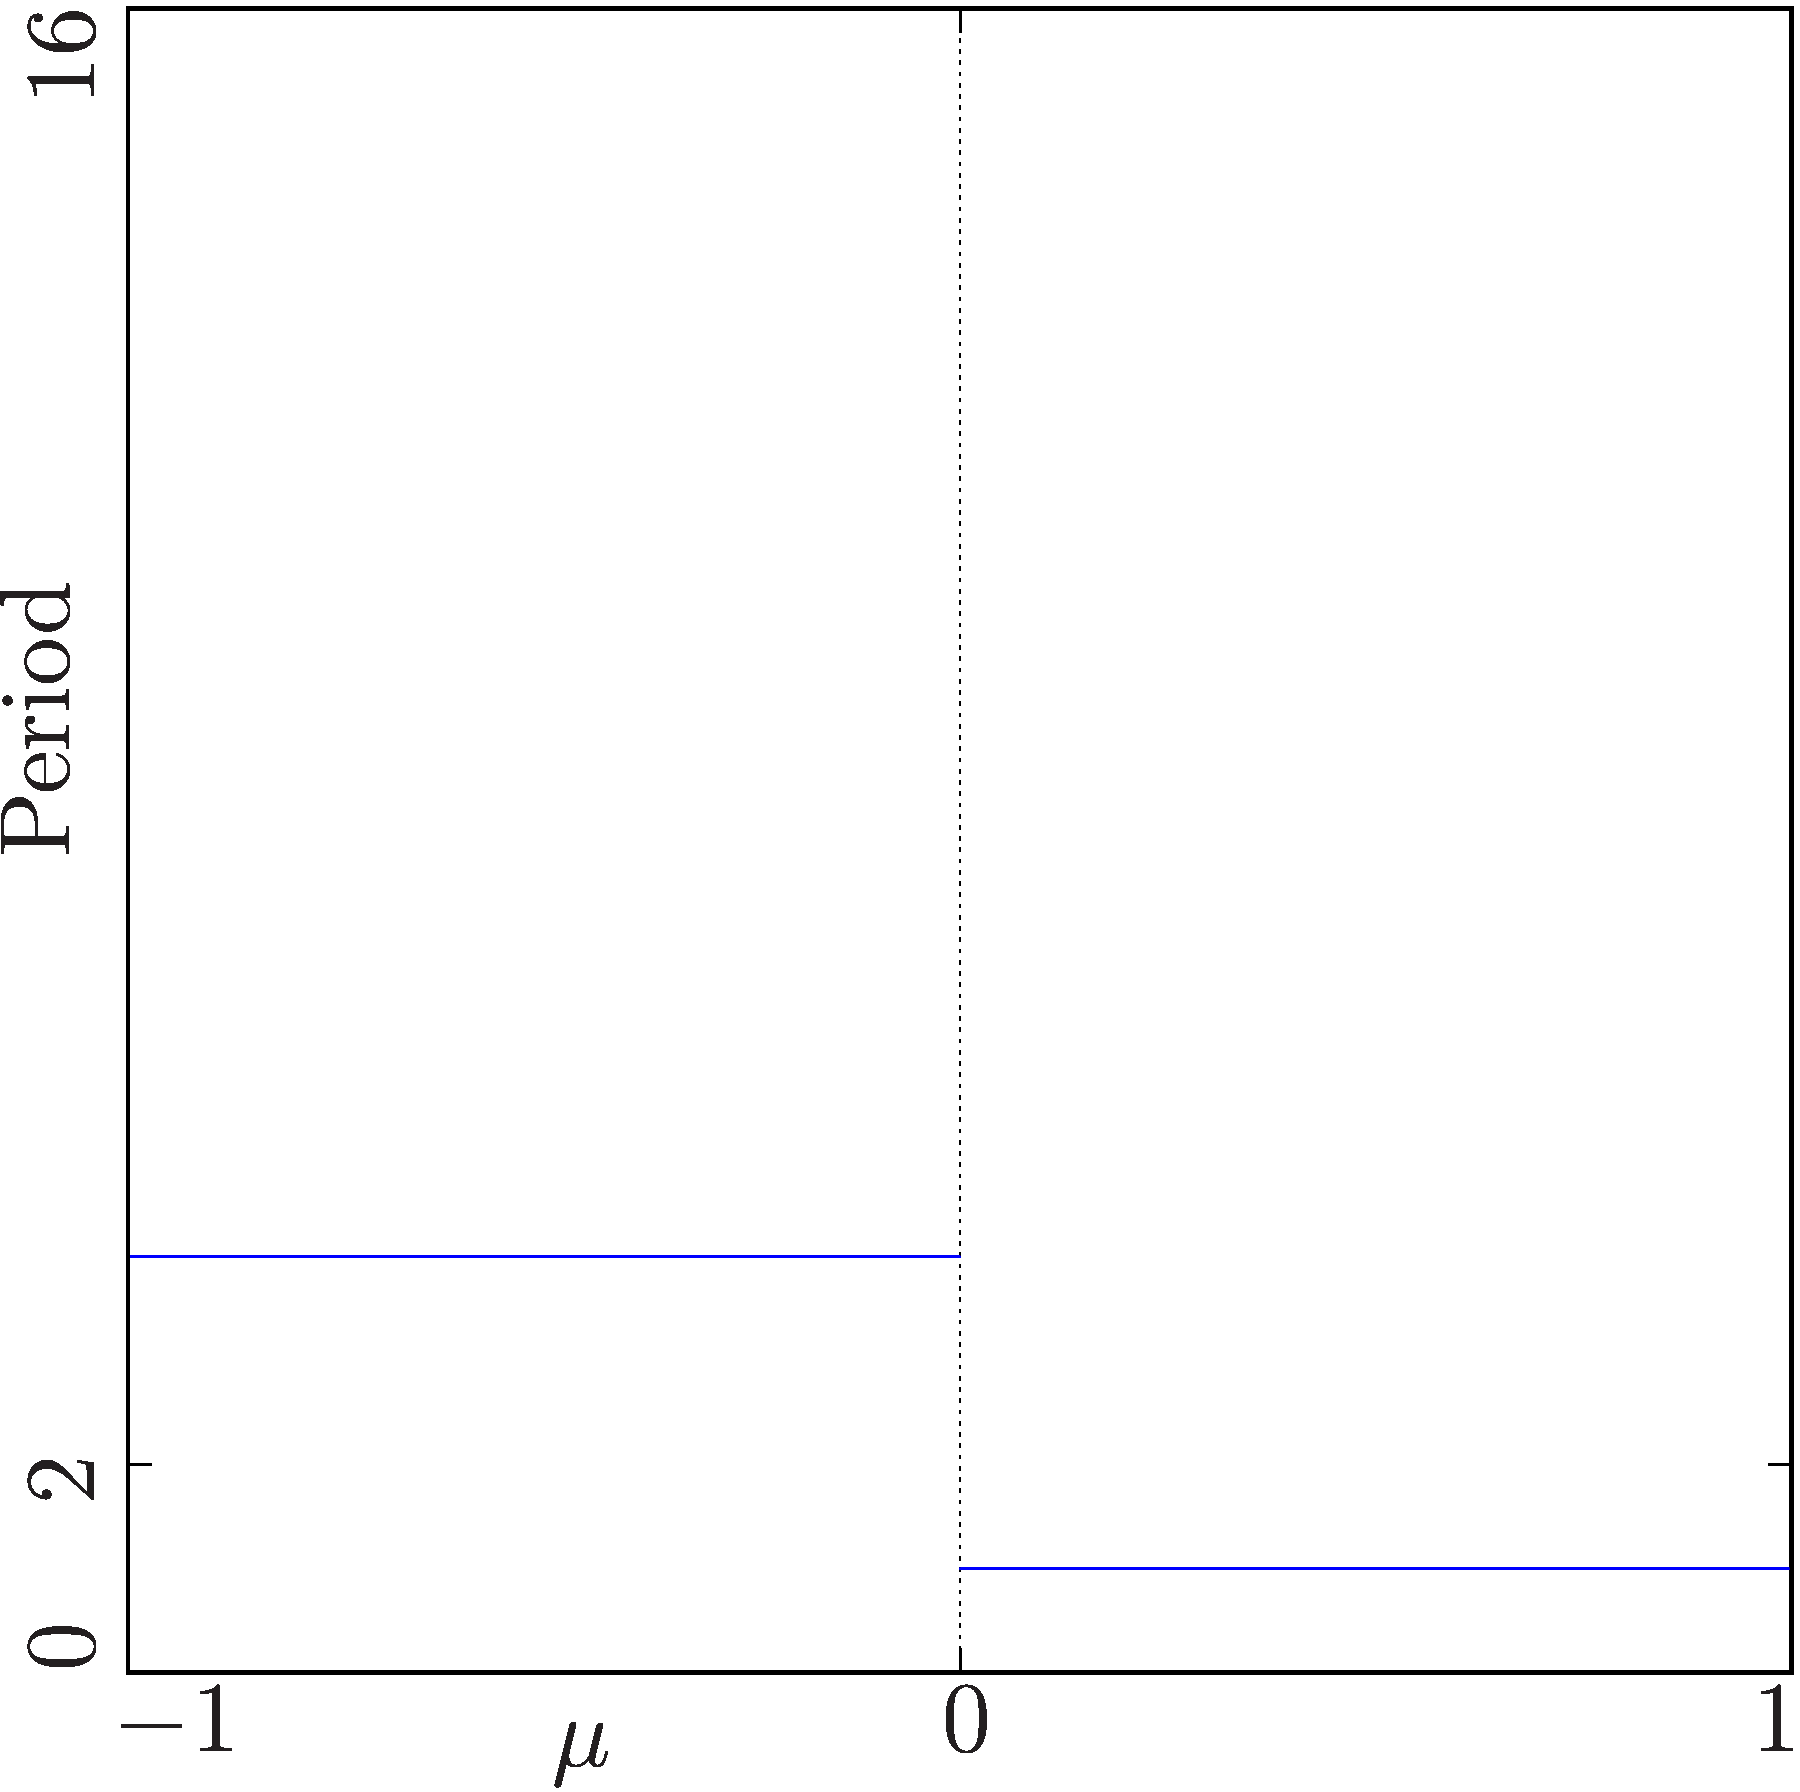
\includegraphics[width=0.6\textwidth]{1D_0b/result.png}
        \caption{Varying $\mu$}
    \end{figure}
\end{frame}

\begin{frame}{(0.b) Fixing $a_L = -2, a_R = 0.5$}
    \begin{figure}
        \centering
            \forloop{n}{0}{\value{n} < 5}{
                \setcounter{f}{\value{n}+1}
                \includegraphics<\arabic{f}>[width=0.6\textwidth]{
                    Cob_0b/Autogen/Frame_00\twodigits{\value{n}}/result.png
                }
            }
        \caption{Cobwebs $\mu \in \{0.01, 0, -0.01, -0.02, -0.03\}$}
    \end{figure}
    
    Absorbing interval: $(-\infty, \infty)$
\end{frame}

\begin{frame}{(0.c) Fixing $a_L = -2, a_R = 0$}
    \begin{figure}
        \centering
        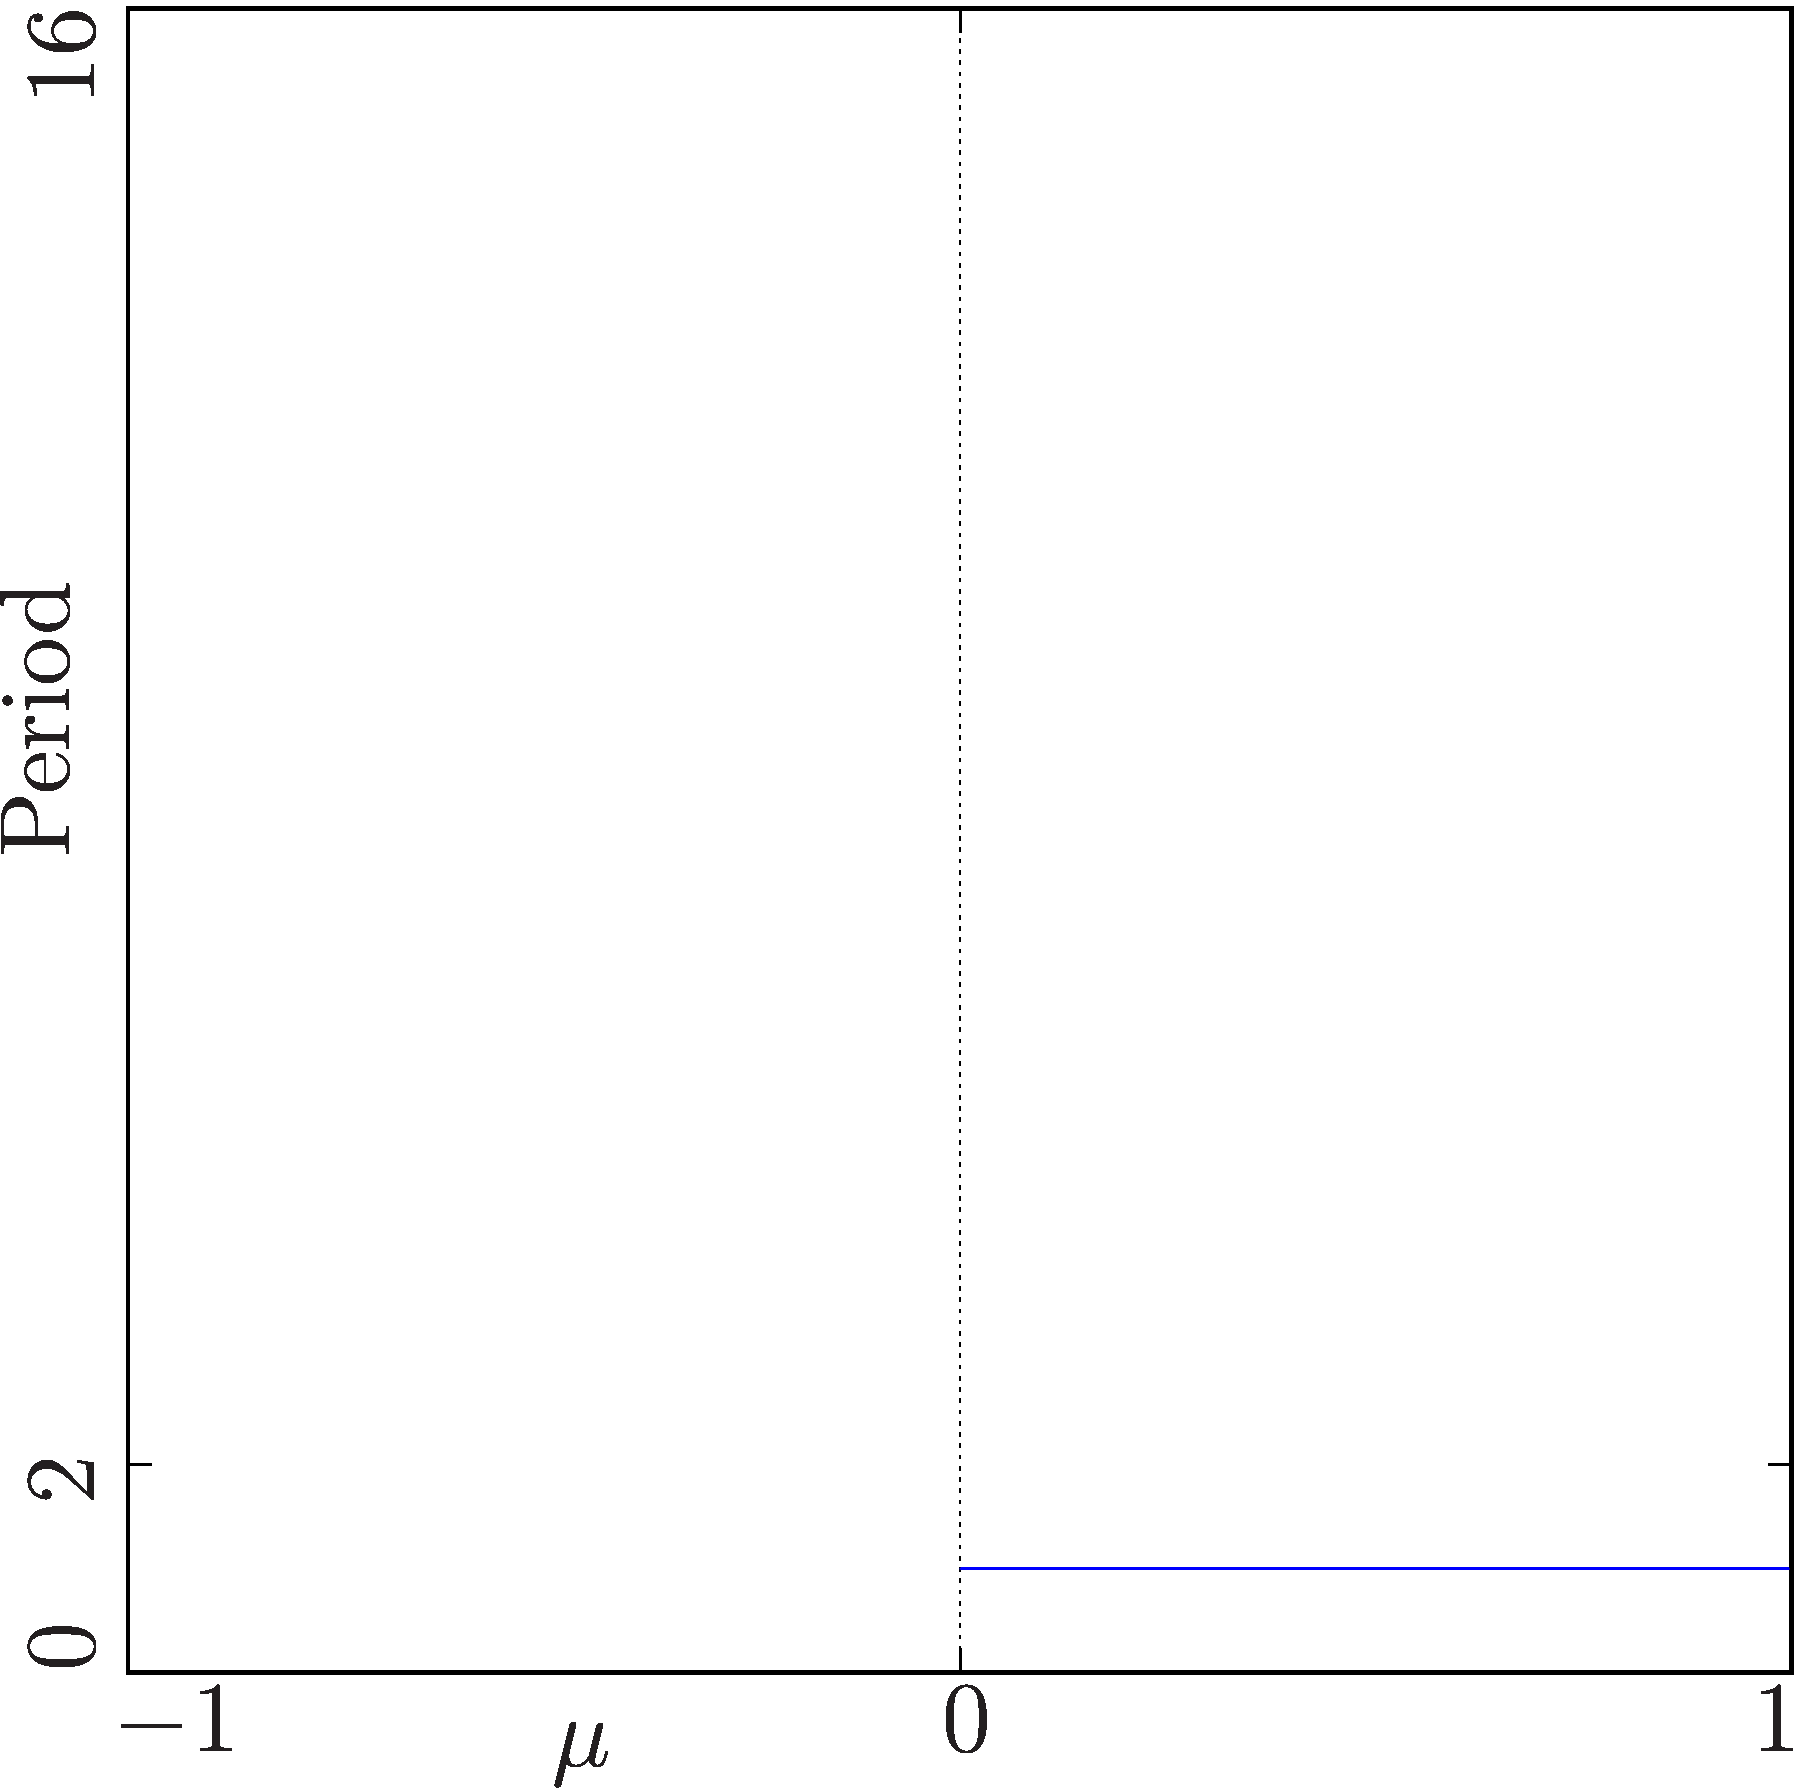
\includegraphics[width=0.6\textwidth]{1D_0c/result.png}
        \caption{Varying $\mu$}
    \end{figure}
\end{frame}

\begin{frame}{(0.b) Fixing $a_L = -2, a_R = 0$}
    \begin{figure}
        \centering
            \forloop{n}{0}{\value{n} < 5}{
                \setcounter{f}{\value{n}+1}
                \includegraphics<\arabic{f}>[width=0.6\textwidth]{
                    Cob_0c/Autogen/Frame_00\twodigits{\value{n}}/result.png
                }
            }
        \caption{Cobwebs $\mu \in \{0.01, 0, -0.01, -0.02, -0.03\}$}
    \end{figure}
    
    Absorbing interval: $(-\infty, \infty)$
\end{frame}

\end{document}
